\chapter{Implementation of Speech Recognition Enhancement using Whisper}

The implementation integrates dataset preparation, augmentation, synthetic data generation, model fine-tuning, and post-processing into a unified pipeline for improving speech recognition on dysarthric speech. The process begins with establishing a baseline performance using a pre-trained model, followed by systematic data enrichment techniques to address variability and scarcity. Advanced augmentation and synthetic audio generation strategies are incorporated to enhance robustness across diverse speech patterns. The refined dataset is then used to fine-tune the model efficiently using parameter-efficient techniques. Finally, an intelligent language model layer is introduced to refine transcriptions and personalize outputs. The chapter concludes with evaluation insights demonstrating significant improvements in recognition accuracy.

\section{Contents of this chapter}
This chapter elaborates the following:
\begin{enumerate}
\item Implementation details for the hardware/software pipeline used in the project
\item Top level design and workflow of the speech recognition enhancement system
\end{enumerate}

\section{System Overview}
The system focuses on improving automatic speech recognition performance for dysarthric speech using a structured pipeline. The implementation is divided into five major components: baseline evaluation, data augmentation, synthetic data generation, model fine-tuning, and language model-based post-processing. Each component contributes to improving the robustness, accuracy, and usability of the system.

\section{Baseline Evaluation}
The initial step involves evaluating the performance of the pre-trained Whisper-base model on the TORGO dataset. The evaluation metric used is Word Error Rate (WER), which quantifies transcription accuracy.

The observed results are:
\begin{itemize}
\item Normalized Overall WER: 0.3215
\item Normalized Dysarthric Speech WER: 0.5994
\item Normalized Healthy Speech WER: 0.1907
\end{itemize}

These results highlight the significant performance gap between healthy and dysarthric speech, motivating the need for further improvements.

\section{Data Augmentation}
To enhance dataset diversity, multiple augmentation techniques are applied to the original audio samples. These transformations simulate real-world variations and improve model robustness.

The augmentation techniques include:
\begin{itemize}
\item Gaussian Noise Injection
\item Pitch Shifting
\item Time Shifting
\item Time Stretching
\end{itemize}

These augmentations are implemented using the \texttt{nlpaug} library, resulting in an expanded dataset with varied acoustic characteristics.

\section{Synthetic Data Generation}
To further address data scarcity, synthetic audio samples are generated using advanced text-to-speech techniques. A custom dataset of textual inputs is used to generate corresponding speech samples.

Key aspects include:
\begin{itemize}
\item Generation of synthetic speech for multiple speakers
\item Balanced dataset creation across gender categories
\item Production of large-scale audio samples in \texttt{.wav} format
\end{itemize}

A total of approximately 16,000 synthetic audio samples are generated, significantly increasing the training data volume and diversity.

\section{Model Fine-Tuning}
The Whisper-base model is fine-tuned using a parameter-efficient approach known as Low-Rank Adaptation (LoRA). This method allows efficient training by updating only a small subset of parameters.

Key implementation details:
\begin{itemize}
\item Fine-tuning performed on approximately 3.6\% of model parameters
\item Integration of augmented and synthetic datasets
\item Optimization focused on improving dysarthric speech recognition
\end{itemize}

This approach reduces computational overhead while maintaining high performance gains.

\section{LLM-based Post Processing}
To further enhance transcription quality, a language model layer is integrated after the speech recognition stage. This component performs grammatical correction and contextual refinement of the generated text.

The post-processing module includes:
\begin{itemize}
\item Correction of grammatical inconsistencies in raw transcriptions
\item Context-aware restructuring of sentences
\item Personalization using a user-specific knowledge base
\end{itemize}

The personalization layer leverages stored contextual information such as frequently used terms, names, or domain-specific vocabulary to produce more meaningful and user-relevant outputs. This significantly improves readability and usability of the transcriptions, especially in assistive communication scenarios.

\section{Top Level Design}
The overall system workflow can be described as a sequential pipeline:

\begin{enumerate}
\item Input Dataset (TORGO Dataset)
\item Baseline Evaluation using Whisper-base
\item Data Augmentation to increase variability
\item Synthetic Data Generation for dataset expansion
\item Dataset Integration and Preprocessing
\item Fine-tuning using LoRA
\item Speech-to-Text Inference
\item LLM-based Post Processing and Personalization
\item Final Output Generation
\end{enumerate}

This pipeline ensures systematic improvement at each stage, leading to better generalization, accuracy, and usability.

\begin{figure}[H]
	\centering
	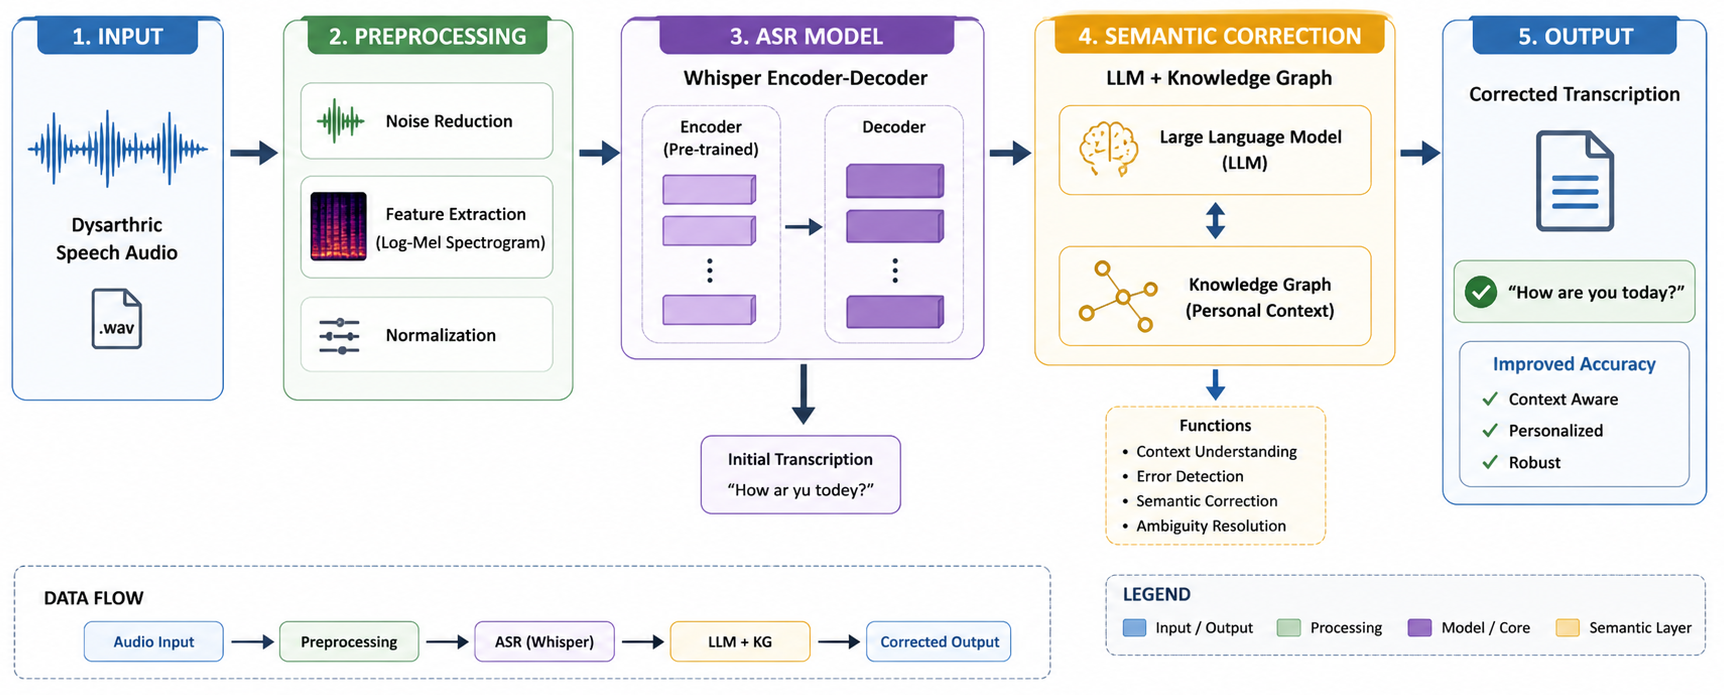
\includegraphics[width=0.9\textwidth]{Figures/architecture_block_diagram.png}
	\caption{System Architecture Block Diagram}
	\label{fig:architecture}
\end{figure}


\section{Performance Evaluation}
After fine-tuning and integrating the post-processing layer, the model is evaluated again on the TORGO dataset using WER as the primary metric. The improved model achieves a WER of less than 20\%, demonstrating a substantial improvement over the baseline.

The reduction in WER, along with improved grammatical coherence and personalization, indicates enhanced recognition capability and overall system effectiveness.

\section{Summary}
The implementation presents a comprehensive pipeline for improving speech recognition performance through both data-centric and model-centric approaches. Starting from baseline evaluation, the system enhances data diversity using augmentation and synthetic generation, followed by efficient fine-tuning. The integration of a language model layer further refines the output by correcting grammar and incorporating personalization. The combined improvements result in significantly better transcription quality and usability. The next chapter focuses on detailed analysis and comparison of results obtained from different configurations and experiments.